\documentclass[9pt]{beamer}
\usepackage[english,bulgarian]{babel}
\usepackage{fontenc}
\usepackage{fontspec}
\usepackage{libertine}

\newfontfamily\fontcomic[NFSSFamily=comic]{Comic Sans MS}

\defaultfontfeatures{Ligatures=TeX}

\usepackage[bulgarian,english]{babel}
\usepackage{indentfirst}
\usepackage{titling}
\usepackage[a4paper, portrait, margin = 2.5 cm]{geometry}
\usepackage{url}
\usepackage{color}
\usepackage{xcolor}
\usepackage{hhline}
\usepackage{xspace}
\usepackage{minibox}
\usepackage{pbox}
\usepackage{mathtools}
\usepackage[framemethod=TikZ]{mdframed}
\usepackage{amsthm}
\usepackage{amssymb}
\usepackage{amsmath}
\usepackage[pdfusetitle]{hyperref}
\usepackage[nameinlink]{cleveref}
\usepackage{mathabx}
\usepackage{graphicx}
\usepackage{ebproof}
\usepackage[toc,page]{appendix}
\usepackage{adjustbox}
\usepackage{lstautogobble}
\usepackage{listings}
\usepackage{syntax}
\usepackage[normalem]{ulem}
\usepackage{subfiles}
\usepackage{csquotes}
\usepackage[style=alphabetic]{biblatex}
\usepackage{tikz-qtree}
\usepackage{tikz}
\usetikzlibrary{fit}
\usetikzlibrary{external}
\usetikzlibrary{positioning}
\tikzset{main node/.style={circle,fill=blue!5,draw,minimum size=1cm,inner sep=0pt},
            }
\tikzset{
    external/system call={%
    xelatex \tikzexternalcheckshellescape
    -halt-on-error -interaction=batchmode -shell-escape
    -jobname "\image" "\texsource"}}
% \tikzexternalize

\newcommand\gderiv{\rightarrow}
\newcommand\gstep{\Rightarrow}
\newcommand\gsteps{\gstep^*}
\newcommand\tderiv{\Rrightarrow}

\newcommand\fun{\rightarrow}
\newcommand\pfun{\mathrel{\ooalign{\hfil$\mapstochar$\hfil\cr$\to$\cr}}}

\renewcommand\descriptionlabel[1]{\qquad $\bullet$ \textbf{#1}}
\newcommand\code[1]{\mbox{\texttt{#1}}}
\newcommand\cendrow{\vspace{0.4em} \\}

\newcommand\note[1]{\marginpar{\scriptsize{ #1 }}}
\newcommand\fixednote[1]{}
\newcommand\discuss[1]{\note{ #1 \textcolor{red}{discuss}}}

\usepackage{color}
\definecolor{Bluish}{rgb}{0.39,0.55,0.78}
\definecolor{exampleness}{HTML}{ebf9d6}
\definecolor{codeness}{HTML}{fbf1c7}
\definecolor{commentness}{HTML}{b57614}
\definecolor{light-gray}{gray}{0.9}
\definecolor{celadon}{rgb}{0.67, 0.88, 0.69}
\definecolor{asparagus}{rgb}{0.53, 0.66, 0.42}
\definecolor{linkness}{rgb}{0.12, 0.43, 0.41}

\newcommand\fixme[1]{
    \greenbox{
        \vspace{1em}
        \textbf{\textcolor{red}{FIXME:} } #1
        \vspace{1em}
    }
}

\newcommand\subtyper[1]{\underline{#1}}
\newcommand\suptyper[1]{\overline{#1}}

\newcommand\catdefsep{\hspace{0.5em} {:} \hspace{0.5em}}
\newcommand\cataddsep{\hspace{0.5em} \phantom{,} \hspace{0.5em}}
\newcommand\termdefsep{\hspace{0.5em} @ \hspace{0.5em}}

\newcommand\mname[1]{\mathrm{#1}}
\newcommand\identity{\mname{id}}

\newcommand\gramshort[1]{
    \begin{alignat*}{2}
        #1
    \end{alignat*}
}

\newcommand\gramrow[3]{
    \ifstrempty{#2}{
        % category is empty, we'll leave just the term
        & \phantom{\catdefsep} & \phantom{\termdefsep} & \quad #3
    }{
        % category is not empty
        \ifstrempty{#1}{
            % token is empty, this is an additional category to the previous token
            \phantom{ } & \cataddsep #2
        }{
            % token is not empty
            #1 &\catdefsep #2
        }
        \ifstrempty{#3}{
            % term is empty
            & \phantom{} & \phantom{}
        }{
            % term is not empty
            & \termdefsep & #3
        }
    } \\
}

\newcommand\plambda[2]{\Lambda^{#2}_{#1}}
\newcommand\fancylambda[2]{\Lambda^{#2}_{\le #1}}
\newcommand\ttlambda[2]{\Lambda^{#2}_{t #1}}
\newcommand\tvlambda[2]{\Lambda^{#2}_{a #1}}
\newcommand\ttt[2]{\langle #1, #2 \rangle}
\newcommand\lattice[2]{\langle #1, #2 \rangle}

\newcommand\betared{\xrightarrow{\beta}}
\newcommand\bbetared{\xRightarrow{\beta}}

\DeclareRobustCommand{\hsout}[1]{\texorpdfstring{\sout{#1}}{#1}}

\renewcommand{\baselinestretch}{1.1}
\setlength{\emergencystretch}{3em}
\setlength{\parskip}{5pt}
\setlength{\parindent}{0pt}

\appto{\bibsetup}{\sloppy}
\addbibresource{references.bib}

\graphicspath{ {./images/} }

\tikzset{%
  boxcola/.style={rectangle,rounded corners,fill=asparagus,draw=asparagus,fill opacity=0.02,thick,inner sep=5pt}
}
\newcommand\boxtexta{asparagus}

\tikzset{%
  boxcolb/.style={rectangle,rounded corners,fill=blue,draw=blue,fill opacity=0.02,thick,inner sep=5pt}
}
\newcommand\boxtextb{blue}

\newcommand\greenbox[1]{
    \tikzexternaldisable
    \begin{samepage}
        \begin{mdframed}[%
            backgroundcolor=green!8,
            linecolor=gray!50!green!60,
            outerlinewidth=0.5pt,
            roundcorner=5mm,
            skipabove=\baselineskip,
            skipbelow=\baselineskip,
            leftmargin=1cm,
            rightmargin=1cm,
        ]
            #1
        \end{mdframed}
    \end{samepage}
    \tikzexternalenable
}

\newenvironment{example}
    {
        \tikzexternaldisable
        \begin{mdframed}[%
            backgroundcolor=exampleness,
            rightline=false,
            topline=false,
            bottomline=false,
            leftline=false,
        ]
            \begin{examplethm}
    }
    {
            \end{examplethm}
        \end{mdframed}
        \tikzexternalenable
    }

\newcommand{\cfigure}[1]{
    \begin{figure}[htbp!]
        \centering
        #1
    \end{figure}
}
\numberwithin{equation}{section}
\numberwithin{figure}{section}
\numberwithin{table}{section}

\newenvironment{lstwrap}
    {
    }
    { 
    }

\lstset{
	backgroundcolor = \color{codeness},
    autogobble,
    columns=fixed,
    showspaces=false,
    showtabs=false,
    breaklines=true,
    showstringspaces=false,
    breakatwhitespace=true,
    escapeinside={(*@}{@*)},
    language=Haskell,
    commentstyle=\color{commentness},
    keywordstyle=\color{black},
    stringstyle=\color{black},
    numberstyle=\color{black},
    basicstyle=\ttfamily\footnotesize,
    frame=lrtb,
    framesep=12pt,
    xleftmargin=12pt,
    xrightmargin=12pt,
    tabsize=4,
    captionpos=b,
    literate={symlambda}{{$\lambda$}}1 {symabstr}{{$\abstr$}}1 {symtot}{{$\tot$}}1
}

\newcommand\restr[2]{{% we make the whole thing an ordinary symbol
  \left.\kern-\nulldelimiterspace % automatically resize the bar with \right
  #1 % the function
  \vphantom{\big|} % pretend it's a little taller at normal size
  \right|_{#2} % this is the delimiter
  }}

\newcommand\tree[1]{
    \begin{tikzpicture}
    \Tree[ #1 ]
    \end{tikzpicture}
}

\newcommand\centree[1]{
    \begin{center}
    \tree{ #1 }
    \end{center}
}

\newcommand\scaledtree[2]{
    \begin{center}
    \begin{tikzpicture}[thick,scale=#1, every node/.style={transform shape}]
    \Tree[ #2 ]
    \end{tikzpicture}
    \end{center}
}

\newcommand\autoscaledtree[1]{
    \begin{center}
    \resizebox{\textwidth}{!}{
        \begin{tikzpicture}
        \Tree[ #1 ]
        \end{tikzpicture}
    }
    \end{center}
}

\newcommand\deriv[1]{
    \begin{prooftree}
        #1
    \end{prooftree}
}

\newcommand\cenderiv[1]{
    \begin{center}
        \deriv{ #1 }
    \end{center}
}

\newcommand\subst[3]{
    #1 [ #2 := #3 ]
}

\hypersetup{
    colorlinks=true,
    linktoc=all,
    citecolor=linkness,
    filecolor=linkness,
    linkcolor=linkness,
    urlcolor=linkness
}

\newcommand\printtoc{
    {
        \hypersetup{linkcolor=black}
        \tableofcontents
    }
}

\usepackage{tabularx}


\setlength{\grammarparsep}{0.2em}
\setlength{\grammarindent}{12em}

\theoremstyle{definition} \newtheorem{convention}{Convention}
                          \numberwithin{convention}{section}
\theoremstyle{definition} \newtheorem{defn}{Definition}
                          \numberwithin{defn}{section}
\theoremstyle{definition} \newtheorem{lemma}{Lemma}
                          \numberwithin{lemma}{section}
\theoremstyle{definition} \newtheorem{prop}{Proposition}
                          \numberwithin{prop}{section}
\theoremstyle{definition} \newtheorem{property}{Property}
                          \numberwithin{property}{section}
\theoremstyle{definition} \newtheorem{examplethm}{Example}
                          \numberwithin{examplethm}{section}
\theoremstyle{definition} \newtheorem{corollary}{Corollary}
                          \numberwithin{corollary}{section}

\newcommand{\lc}{\textcolor{red}{\backslash}}
\newcommand{\rc}{\textcolor{red}{/}}
\newcommand{\mc}{\textcolor{red}{|}}
\newcommand{\lci}[1]{\textcolor{red}{\backslash_{#1}}}
\newcommand{\rci}[1]{\textcolor{red}{/_{#1}}}
\newcommand{\mci}[1]{\textcolor{red}{|_{#1}}}
\newcommand{\lb}{\textcolor{red}{[}}
\newcommand{\rb}{\textcolor{red}{]}}
\newcommand{\lp}{\textcolor{red}{(}}
\newcommand{\rp}{\textcolor{red}{)}}
\newcommand{\modstar}{\star}
\newcommand{\moddot}{.}
\newcommand{\modr}{\lozenge}
\newcommand{\modx}{\times}

\newcommand{\meet}{\wedge}
\newcommand{\join}{\vee}
\newcommand{\unify}{\hat{\wedge}}
\newcommand{\less}{\leq}
\newcommand{\termless}[2]{\less_{ #1 }^{ #2 }}
\newcommand{\termlessne}[2]{<_{ #1 }^{ #2 }}
\newcommand{\termlen}[1]{| #1 |}
\newcommand{\lesss}{\ll}
\newcommand{\lass}{<:}
\newcommand{\tless}{\sqsupseteq}

\renewcommand{\land}{\mathbin{\&}}
\newcommand{\xor}{\veebar}
\newcommand{\boolset}{\mathbb{B}}

\newcommand{\mcf}[1]{\mathsf{#1}}

\newcommand{\tclos}[1]{\mathcal{T}( #1 )}
\newcommand{\tvclos}[1]{\mathcal{T}_v( #1 )}
\newcommand{\cclos}[1]{\mathcal{C}( #1 )}
\newcommand{\catsin}[1]{\mathsf{Cats}( #1 )}
\newcommand{\tsymbs}{\mathbb{T}}
\newcommand{\csymbs}{\mcf{Cat}}
\newcommand{\lvars}{\mathbb{V}^{\lambda}}
\newcommand{\cvars}{\mathbb{V}^{C}}
\newcommand{\tvars}{\mathbb{V}^{T}}
\newcommand{\trees}[1]{\mathbb{T}_{ #1 }}
\newcommand{\const}{\mcf{Const}}
\newcommand{\fvv}{\mcf{fv}}
\newcommand{\fv}[1]{\fvv(#1)}
\newcommand{\tss}{\mcf{ts}}
\newcommand{\ts}[1]{\tss(#1)}

\newcommand{\squash}{\omega}
\newcommand{\consquash}{\squash^{\gamma}}
\newcommand{\lsquash}{\squash^{\lambda}}
\newcommand{\tsquash}{\hat{\squash}}

\newcommand{\tadd}{\oplus}
\newcommand{\tot}{\rightarrow}
\newcommand{\abstr}{\Rightarrow}
\newcommand{\app}{\text{ }}
\newcommand{\sq}{\text{ }}
\newcommand{\wildcard}{\Asterisk}
\newcommand{\typeof}[1]{\|#1\|}
\newcommand{\typeoff}{\typeof{\cdot}}
\newcommand{\typeofv}[1]{\typeof{#1}_v}
\newcommand{\typeofvv}{\typeofv{\cdot}}
\newcommand{\defeq}{\overset{\text{\scriptsize def}}{=}}
\newcommand{\defiff}{\overset{\text{\scriptsize def}}{\iff}}
\newcommand{\condeq}{\simeq}

\newcommand{\latex}{\LaTeX\xspace}

\usetheme{metropolis}
% \usecolortheme{dove}
\title{Катег\'орийни граматики за геопространствени заявки}
\date{\today}
\author{Бла Бла}
\institute{Магистър университет ФМИ бла}
\begin{document}
  \maketitle

  \section{Геопространствени заявки}
  \begin{frame}[fragile]
    Вход:
    \begin{lstwrap}\begin{lstlisting}
      pharmacies near parking spaces in Berlin
    \end{lstlisting}\end{lstwrap}
    Изход:

    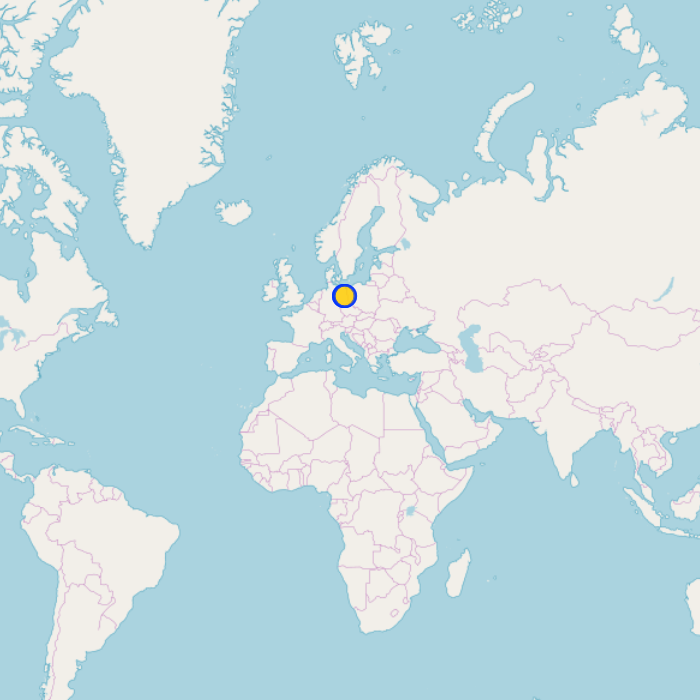
\includegraphics[width=0.32\textwidth]{map/world.png}
    \hfill
    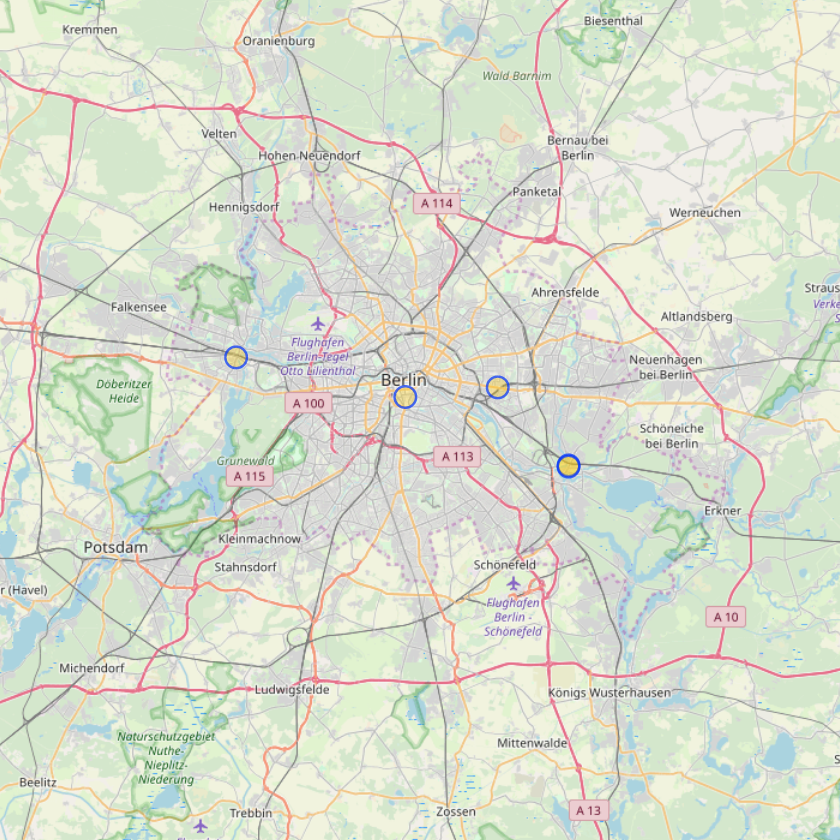
\includegraphics[width=0.32\textwidth]{map/berlin.png}
    \hfill
    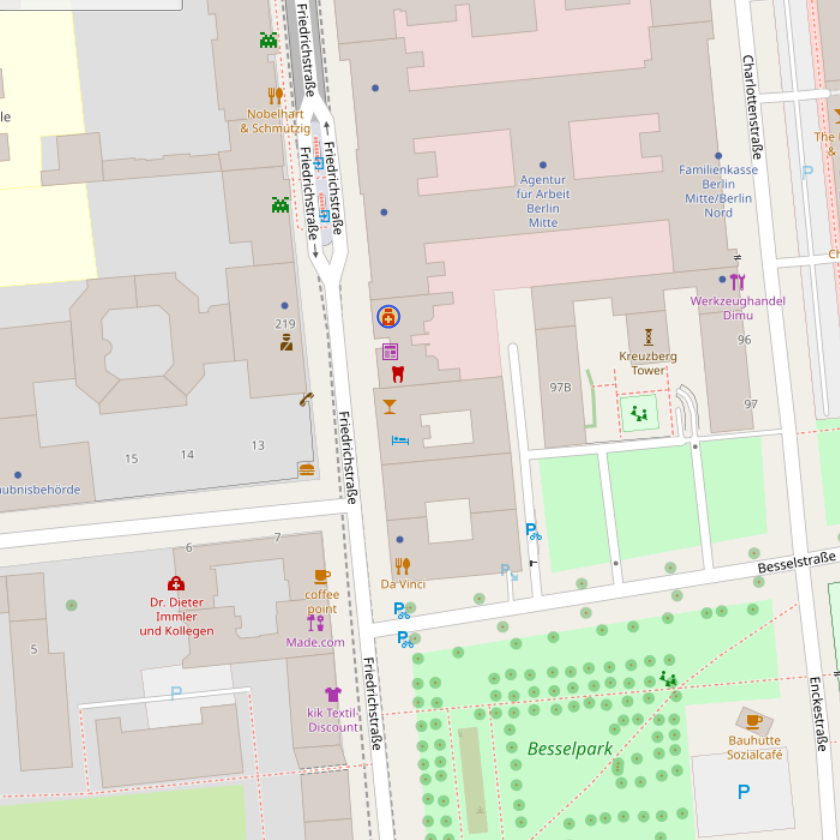
\includegraphics[width=0.32\textwidth]{map/pharmacy.png}
  \end{frame}

  \section{Overpass}
  \begin{frame}[fragile]{Overpass код}
    \begin{lstwrap}\begin{lstlisting}
    ( node["amenity" = "parking_space"]; ) -> .x1;
    ( area["name" = "Berlin"]; area["int_name" = "Berlin"]; area["name:en" = "Berlin"]; ) -> .x2;
    ( node(area.x2)(around.x1:100.0)["amenity" = "pharmacy"]; ) -> .x3;
    .x3 out;
    \end{lstlisting}\end{lstwrap}
  \end{frame}

  \begin{frame}{Типове обекти в Overpass}
    \begin{itemize}
      \item node
      \item way
      \item relation
      \item area
    \end{itemize}
  \end{frame}

  \begin{frame}{Set}

  \end{frame}

  \begin{frame}[fragile]{Резултат от заявка}
    \begin{lstwrap}\begin{lstlisting}
        out <input set>;
    \end{lstlisting}\end{lstwrap}
  \end{frame}

  \begin{frame}[fragile]{Извличане на обекти}
    \begin{itemize}
      \item Синтаксис
        \begin{lstwrap}\begin{lstlisting}
            <object keyword><filter><filter>...<filter>
        \end{lstlisting}\end{lstwrap}
      \item Пример
        \begin{lstwrap}\begin{lstlisting}
            node[name="Foo"];
            out;
        \end{lstlisting}\end{lstwrap}
        \begin{lstwrap}\begin{lstlisting}
            node[name="Foo"] -> ._;
            out ._;
        \end{lstlisting}\end{lstwrap}
    \end{itemize}
  \end{frame}

  \begin{frame}[fragile]{Извличане на обекти}
    \begin{itemize}
      \item Синтаксис
        \begin{lstwrap}\begin{lstlisting}
            <keyword><filter><filter>...<filter>
        \end{lstlisting}\end{lstwrap}
      \item Ключови думи
        \begin{center}
            \begin{tabular}{r|l}
                \code{node} & retrieves nodes \\
                \code{way} & retrieves ways \\
                \code{relation} & retrieves relations \\
                \code{area} & retrieves areas \\
                \code{nwr} & retrieves nodes, ways, and relations \\
            \end{tabular}
        \end{center}
    \end{itemize}
  \end{frame}

  \begin{frame}[fragile]{Други филтри за ``тагове''}
    \begin{lstwrap}\begin{lstlisting}
        node[amenity="cafe"];
    \end{lstlisting}\end{lstwrap}

    \begin{lstwrap}\begin{lstlisting}
        node[amenity="cafe"][name="Moondeers"];
    \end{lstlisting}\end{lstwrap}

    \begin{lstwrap}\begin{lstlisting}
        node[amenity="cafe"][name~"^moondeers$",i];
    \end{lstlisting}\end{lstwrap}

    \begin{lstwrap}\begin{lstlisting}
        area["administrative"];
    \end{lstlisting}\end{lstwrap}
  \end{frame}

  \begin{frame}[fragile]{Сечение}
      \begin{lstwrap}\begin{lstlisting}
          node[amenity="cafe"] -> .cafes;
          node.cafes;
      \end{lstlisting}\end{lstwrap}
      \begin{lstwrap}\begin{lstlisting}
          node[amenity="cafe"] -> .cafes;
          node.cafes[name="Moondeers"];
      \end{lstlisting}\end{lstwrap}
  \end{frame}

  \begin{frame}[fragile]{Обекти в area}
    \begin{lstwrap}\begin{lstlisting}
      area[name="Frankfurt"] -> fr;
      node(area.fr);
      out;
    \end{lstlisting}\end{lstwrap}
  \end{frame}

  \begin{frame}[fragile]{Обекти на разстояние от други обекти}
    \begin{lstwrap}\begin{lstlisting}
        node[amenity="parking_space"] -> pspaces;
        node[amenity="cafe"](around.pspaces:120) -> x;
        out x;
    \end{lstlisting}\end{lstwrap}
    \begin{lstwrap}\begin{lstlisting}
        area[name="Bonn"];
        node(area)[highway=bus_stop];
        node(around:100)[amenity=cinema];
        out;
    \end{lstlisting}\end{lstwrap}
  \end{frame}

  \begin{frame}[fragile]{Обединение}
    \begin{lstwrap}\begin{lstlisting}
        node[amenity="cafe"] -> .cafes;
        area[name="Bonn"] -> .bonn;
        area[name="Frankfurt"] -> .frankfurt;
        node.cafes(area.bonn) -> .cb;
        node.cafes(area.frankfurt) -> .cf;
        (.cf; .cb;) -> .cfb;
        out .cfb;
    \end{lstlisting}\end{lstwrap}

    \begin{lstwrap}\begin{lstlisting}
        area[name="Bonn"] -> .bonn;
        area[name="Frankfurt"] -> .frankfurt;
        ( node[amenity="cafe"](area.bonn); node[amenity="cafe"](area.frankfurt); );
        out;
    \end{lstlisting}\end{lstwrap}
  \end{frame}

  \section{Типово $\lambda$-смятане}
  \begin{frame}{$\lambda$}няколко слайда тук\end{frame}

  \section{Minipass: междинен език}
  \begin{frame}{Графова абстракция}
    \begin{itemize}
      \item Върхове: Overpass обекти
        \begin{itemize}
          \item по тип
          \item по стойност на таг (например име)
          \item ...
        \end{itemize}
      \item Ребра: връзки между обектите \pika
        \begin{itemize}
          \item близост
          \item физическо съдържане
          \item ...
        \end{itemize}
    \end{itemize}
  \end{frame}

  \begin{frame}[fragile]{Графова абстракция: пример}
    Заявка:
    \begin{lstwrap}\begin{lstlisting}
      bus stops near schools in Russia
    \end{lstlisting}\end{lstwrap}

    \begin{enumerate}
      \item Нека $B$ е множеството от върховете, имащи етикет
        ``е автобусна спирка''
      \item Нека $S$ е множеството от върховете, имащи етикет
        ``е училище''
      \item Нека $R$ е множеството от върховете, имащи етикет
        ``английското му име е \emph{Russia}''
      \item Нека $N$ е множеството от върховете, които можем да
        достигнем от върхове в $S$, ходейки по ребро, имащо етикет
        ``е близо до''
      \item Нека $P$ е множеството от върховете, които можем да
        достигнем от върхове в $R$, ходейки по ребро, имащо етикет
        ``е във вътрешността на''
      \item Резултатът е $B \cap N \cap P$.
    \end{enumerate}
  \end{frame}

  \begin{frame}{Синтаксис: Основни типове}
    \begin{itemize}
      \item $Num$ - цяло число \pika
      \item $String$ - низ \pika
      \item $List$ - полиморфен свързан списък, който може
        да съдържа $Num$, $String$ и $List$
      \item $GSet$ - множество от географски обекти: съответства на \code{Set}
        в Overpass
    \end{itemize}
  \end{frame}

  \begin{frame}{Синтаксис: $\lambda$}
    \begin{itemize}
      \item Прилагане на термове (ляво-асоциативно)
        \begin{center}
          \code{<term1> <term2>}
        \end{center}
      \item Абстракция
        \begin{center}
          \code{lambda <varname> : <type> => <term>}
        \end{center}
      \item Променливи и константи
      \item Сложни типове
        \begin{center}
          \code{<type1> -> <type2>}
        \end{center}
    \end{itemize}
  \end{frame}

  \begin{frame}{Синтаксис: ключови думи}
    \begin{center}
      \begin{tabular}{r l p{0.35\textwidth}}
        Идентификатор  & Тип & \\
        \hline
        \code{and}  & $GSet \tot GSet \tot GSet$ & сечение \cendrow
        \code{or}   & $GSet \tot GSet \tot GSet$ & обединение \cendrow
        \code{not}  & $GSet \tot GSet$ & допълнение \cendrow
        \hline
        \code{get}  & $List \tot GSet$ & извличане на географски обекти по
        етикет на връх \cendrow
        \code{next} & $List \tot GSet \tot GSet$ & извличане на географски обекти
        траверсирайки ребро \cendrow
      \end{tabular}
    \end{center}
  \end{frame}
  \begin{frame}{Синтаксис: ключови думи за списъци}
    \begin{center}
      \begin{tabular}{r l p{0.35\textwidth}}
        Идентификатор  & Тип & \\
        \hline
        \code{empty} & $List$ & празен списък \cendrow
        \code{consNum} & $Num \tot List \tot List$ & залепяне на число
        в началото на списък \cendrow
        \code{consString} & $String \tot List \tot List$ & залепяне на низ
        в началото на списък \cendrow
        \code{consList} & $List \tot List \tot List$ & залепяне на списък
        в началото на списък \cendrow
      \end{tabular}
    \end{center}
  \end{frame}

  \begin{frame}[fragile]{Пример}
    Искаме да извадим всички училища, физически намиращи се в обекти,
    които се казват Sofia:
    \begin{lstwrap}\begin{lstlisting}
and
    (get (consString 'tagFilter'
            (consList (consString '='
                (consString 'amenity'
                    (consString 'school' empty)))
        empty)))
    (next (consString 'in' empty)
        (get (consString 'tagFilter' (consList
            (consString '='
                (consString 'name'
                    (consString 'Sofia' empty)))
        empty))))
    \end{lstlisting}\end{lstwrap}
  \end{frame}

  \begin{frame}[fragile]{``Стандартна'' библиотека}
    \begin{lstwrap}\begin{lstlisting}
      -- get all items of given type
      nodes     :=  get (consString 'all'
      (consString 'nodes' empty)).
      ways      :=  get (consString 'all'
      (consString 'ways' empty)).
      relations :=  get (consString 'all'
      (consString 'relations' empty)).
      areas     :=  get (consString 'all'
      (consString 'areas' empty)).

      -- get all items in the universe
      everything := get (consString 'all' empty).
    \end{lstlisting}\end{lstwrap}
  \end{frame}

  \begin{frame}[fragile]{``Стандартна'' библиотека}
    \begin{lstwrap}\begin{lstlisting}
-- find items by tag key and value infix
contains  :=  \k: String, n: String => get
    (consString 'tagFilter'
        (consList (consString '~'
            (consString k (consString n empty)))
        empty)).

-- find items within distance of given items
within    :=  \dist : Num => next
    (consString 'around' (consNum dist empty)) .

-- find items inside of given items
in        :=  next (consString 'in' empty).
    \end{lstlisting}\end{lstwrap}
  \end{frame}
  \begin{frame}[fragile]{``Стандартна'' библиотека}
    \begin{lstwrap}\begin{lstlisting}
-- find items by name
name      :=  \x => or (or
        (kv 'name' x)
        (kv 'int_name' x))
    (kv 'name:en' x).

-- find items by name infix
nameLike  :=  \x => or (or
        (contains 'name' x)
        (contains 'int_name' x))
    (contains 'name:en' x).

-- find items by amenity key (fountain, school...)
amenity   :=  kv 'amenity'.

-- find items by tag key and value
kv        :=  \k: String, n: String => get
    (consString 'tagFilter'
        (consList (consString '='
            (consString k (consString n empty)))
    empty)).
    \end{lstlisting}\end{lstwrap}
  \end{frame}
  \begin{frame}[fragile]{``Стандартна'' библиотека}
    \begin{lstwrap}\begin{lstlisting}
-- identity
id        := \y => y.

-- the set of all cities
city      := or (or
        (kv 'admin_level' '8')
        (kv 'admin_level' '6'))
    (kv 'capital' '4').

-- within 100 metres
near      :=  within 100.
    \end{lstlisting}\end{lstwrap}
  \end{frame}

  \begin{frame}[fragile]{Пример (отново)}
    Искаме да извадим всички училища, физически намиращи се в обекти,
    които се казват Sofia:
    \begin{lstwrap}\begin{lstlisting}
and (amenity 'school') (in (name 'Sofia'))
    \end{lstlisting}\end{lstwrap}
  \end{frame}


  \section{Подтипове}
  \begin{frame}{Подтипове}няколко слайда тук\end{frame}

  \section{Категорийни граматики}
  \begin{frame}{Категорийни граматики: пример}
    \code{pharmacies near parking spaces in Berlin}
  \end{frame}

  \begin{frame}{Категорийни граматики: пример}
    \gramshort{
        \gramrow{pharmacies}{ GSet }{}
        \gramrow{Berlin}{ GSet }{}
    }
  \end{frame}
  \begin{frame}{Категорийни граматики: пример}
    \gramshort{
        \gramrow{pharmacies}{ GSet }{}
        \gramrow{Berlin}{ GSet }{}
        \gramrow{parking}{ GSet \rc Spaces }{}
        \gramrow{spaces}{Spaces}{}
    }
  \end{frame}
  \begin{frame}{Категорийни граматики: пример}
    \gramshort{
        \gramrow{pharmacies}{ GSet }{}
        \gramrow{Berlin}{ GSet }{}
        \gramrow{parking}{ GSet \rc Spaces }{}
        \gramrow{spaces}{Spaces}{}
        \gramrow{in}{ (GSet \lc GSet) \rc GSet }{}
        \gramrow{near}{ (GSet \lc GSet) \rc GSet }{}
    }
  \end{frame}
  \begin{frame}{Категорийни граматики: пример}
    \autoscaledtree{.{$GSet$}
        [ .{$GSet$}
            [ .{$GSet$} [ .{$pharmacies$} ] ]
            \edge[very thick];
            [ .{$GSet \lc GSet$}
                \edge[very thick];
                [ .{$(GSet \lc GSet) \rc GSet$} [ .{$near$} ] ]
                [ .{$GSet$}
                    \edge[very thick];
                    [ .{$GSet \rc Spaces$} [ .{$parking$} ] ]
                    [ .{$Spaces$} [ .{$spaces$} ] ]
                ]
            ]
        ]
        \edge[very thick];
        [ .{$GSet \lc GSet$}
            \edge[very thick];
            [ .{$(GSet \lc GSet) \rc GSet$} [ .{$in$} ] ]
            [ .{$GSet$} [ .{$Berlin$} ] ]
        ]
    }
  \end{frame}

  \section{Категорийни граматики (формално)}
  \begin{frame}{Категорийно затваряне}
    \begin{enumerate}
        \item \label{itm:atomic} $A \in \tau \implies A \in \cclos{\tau}$
        \item \label{itm:right}  $X, Y \in \cclos{\tau} \implies \lp X \rc Y \rp \in \cclos{\tau}$
        \item \label{itm:left}   $X, Y \in \cclos{\tau} \implies \lp X \lc Y \rp \in \cclos{\tau}$
    \end{enumerate}
  \end{frame}

  \begin{frame}{(Чиста) категорийна граматика}
    $ G = \langle \Sigma, N, S, f, n \rangle $ е \emph{категорийна граматика}, ако
    \begin{itemize}
        \item $ \Sigma $ е крайно множество от \emph{терминали}
        \item $ N $ е крайно множество от \emph{нетерминали} (атомарни категории)
        \item $ S \in N $
        \item $ f : \Sigma \fun \hat{N} $, където $\hat{N}$ е множеството от
            \textbf{крайни} подмножества на $\cclos{N}$
        \item $ n \in \mathbb{N} $
    \end{itemize}
  \end{frame}

  \begin{frame}{Правила за извод}
    \begin{itemize}
        \item Ако $ a \in \Sigma, X \in f(a) $, то \[ \lb X \rb \gderiv_G a \]
        \item Ако $ X \rc Y \in \cclos{N}, Y \mci{1} Z_1 \mci{2} Z_2 ... \mci{m} Z_m \in \cclos{N}, 0 \leq m \leq n $
            то \[ \lb X \mci{1} Z_1 \mci{2} Z_2 ... \mci{m} Z_m \rb \gderiv_G \lb X \rc Y \rb \lb Y \mci{1} Z_1 \mci{2} Z_2 ... \mci{m} Z_m \rb \]
        \item Ако $ X \lc Y \in \cclos{N}, Y \mci{1} Z_1 \mci{2} Z_2 ... \mci{m} Z_m \in \cclos{N}, 0 \leq m \leq n $
            то \[ \lb X \mci{1} Z_1 \mci{2} Z_2 ... \mci{m} Z_m \rb \gderiv_G \lb Y \mci{1} Z_1 \mci{2} Z_2 ... \mci{m} Z_m \rb \lb X \lc Y \rb \]
    \end{itemize}
  \end{frame}

  \begin{frame}{Пример}
    Ще построим проста граматика $G = \langle \Sigma, N, S, f, n \rangle$
    която генерира \code{cities in Germany}:

    \begin{align*}
        \Sigma \defeq& \{ cities, in, Germany \} \\
        N \defeq& \{ GSet \} \\
        S \defeq& GSet \\
        f(x) \defeq&
            \begin{cases*}
                \{ GSet \},& x = cities \\
                \{ GSet \},& x = Germany \\
                \{ GSet \lc GSet \rc GSet \},& x = in \\
            \end{cases*} \\
        n \defeq& 1 \\
    \end{align*}
  \end{frame}

  \begin{frame}{Примерен извод}
    \begin{center}
        \begin{tabular}{c}
            $\underline{\lb GSet \rb}$ \\ $\gstep$ \\
            $\lb GSet \rb \underline{\lb GSet \lc GSet \rb}$ \\ $\gstep$ \\
            $\underline{\lb GSet \rb} \lb GSet \lc GSet \rc GSet \rb \lb GSet \rb$ \\ $\gstep$ \\
            $cities \sq \underline{\lb GSet \lc GSet \rc GSet \rb} \lb GSet \rb$ \\ $\gstep$ \\
            $cities \sq in \sq \underline{\lb GSet \rb}$ \\ $\gstep$ \\
            $cities \sq in \sq Germany$ \\
        \end{tabular}
    \end{center}
  \end{frame}

  \begin{frame}{Свойство}
    Всяка КГ $G = \langle \Sigma, N, S, f, n \rangle$ е еквивалентна на
    (безкрайна) контекстно свободна граматика
    $G^C = \langle \Sigma, \lb \cclos{N} \rb, R, \lb S \rb \rangle$.

    Освен това, имайки извод $\mu: \alpha_1 \gstep ... \gstep \alpha_r$.
    Можем да построим специална \textbf{крайна} контекстно-свободна граматика
    $G_\mu^C = \langle \Sigma, \lb \catsin{\mu} \rb, \restr{R}{\lb \catsin{\mu} \rb}, \lb S \rb \rangle$,
    в която $\mu$ е валиден извод и всички нейни изводи са изводи и в $G$.

    \begin{proof}
        Дефинициите на $\gstep$ за $G$ и за $G^C$ съвпадат.
    \end{proof}
  \end{frame}

  \begin{frame}{CYK за КГ}
    По даден вход (дума) строим строим множество $P$ от тройки
    $(X, i, j)$, $X \in \cclos{N}, 1 \leq i \leq j \leq k$ индуктивно,
    опитвайки се да получим
    $(S, 1, k)$.

    \begin{enumerate}
    \label{cyk:rules}
        \item Ако $X \in f(w_i)$, то $(X, i, i) \in P$.
        \item Ако $(X \rc Y, i, p) \in P, (Y \mci{1} Z_1 \mci{2} Z_2 ... \mci{m} Z_m, p + 1, j) \in P$,
            то $(X \mci{1} Z_1 \mci{2} Z_2 ... \mci{m} Z_m, i, j) \in P$.
        \item Ако $(X \lc Y, p + 1, j) \in P, (Y \mci{1} Z_1 \mci{2} Z_2 ... \mci{m} Z_m, i, p) \in P$,
            то $(X \mci{1} Z_1 \mci{2} Z_2 ... \mci{m} Z_m, i, j) \in P$.
    \end{enumerate}
  \end{frame}

  \begin{frame}{Коректност}
    \begin{enumerate}
        \item Ако $X \in f(w_i)$, то $(X, i, i) \in P$.
        \item Ако $(X \rc Y, i, p) \in P, (Y \mci{1} Z_1 \mci{2} Z_2 ... \mci{m} Z_m, p + 1, j) \in P$,
            то $(X \mci{1} Z_1 \mci{2} Z_2 ... \mci{m} Z_m, i, j) \in P$.
        \item Ако $(X \lc Y, p + 1, j) \in P, (Y \mci{1} Z_1 \mci{2} Z_2 ... \mci{m} Z_m, i, p) \in P$,
            то $(X \mci{1} Z_1 \mci{2} Z_2 ... \mci{m} Z_m, i, j) \in P$.
    \end{enumerate}

    \begin{equation}\label{eq:left}
        (X, i, j) \in P \implies \lb X \rb \gsteps w_i ... w_j
    \end{equation}
  \end{frame}
  \begin{frame}{Пълнота}
    \begin{enumerate}
        \item Ако $X \in f(w_i)$, то $(X, i, i) \in P$.
        \item Ако $(X \rc Y, i, p) \in P, (Y \mci{1} Z_1 \mci{2} Z_2 ... \mci{m} Z_m, p + 1, j) \in P$,
            то $(X \mci{1} Z_1 \mci{2} Z_2 ... \mci{m} Z_m, i, j) \in P$.
        \item Ако $(X \lc Y, p + 1, j) \in P, (Y \mci{1} Z_1 \mci{2} Z_2 ... \mci{m} Z_m, i, p) \in P$,
            то $(X \mci{1} Z_1 \mci{2} Z_2 ... \mci{m} Z_m, i, j) \in P$.
    \end{enumerate}
    \begin{equation}\label{eq:right}
        \lb X \rb \gsteps w_i ... w_j \implies (X, i, j) \in P
    \end{equation}
  \end{frame}

  \begin{frame}{Семантика в КГ}
    Дефинираме $\typeoff : \cclos{N} \fun \tclos{\Theta}$ като:
    \[\typeof{\lp X \mc Y \rp} \defeq  \typeof{Y} \tot \typeof{X}\].

    По дадена КГ $ G = \langle \Sigma, N, S, f, n \rangle $, функцията
    \[ \psi : \{ (a, X) \mid a \in \Sigma, X \in f(a) \} \fun 2^{\plambda{\Theta}{C}} \]
    ще наричаме \emph{семантична функция} за $G$.
  \end{frame}

  \begin{frame}{Семантика в КГ: базов случай}
    \begin{center}
        \begin{tikzpicture}[node distance=1mm,sibling distance=1cm]
            \Tree[
                .\node(outtop){$X$};
                    \edge[very thick];
                    [ .\node(in){$a$};
                    ]
            ]
            \node[boxcolb,fit=(outtop)(in)](outbox){};
            \node[right=of outbox,text=\boxtextb](outlabel){$T$};
        \end{tikzpicture}
    \end{center}
    \[ X \in f(a) \]
    \hrule
    \[ sem_{\psi}(T) = \psi(a, X). \]
  \end{frame}

  \begin{frame}{Семантика в КГ: десен случай}
    \begin{center}
      \begin{tikzpicture}[node distance=1mm,sibling distance=1cm]
        \Tree[
        .\node(outtop){$X \mci{1} Z_1 \mci{2} Z_2 ... \mci{m} Z_m$};
        \edge[very thick];
        [ .\node(intopl){$X \rc Y$};
        \edge[roof];
        [ .\node(inbotl){$\alpha$}; ]
        ]
        [ .\node(intopr){$Y \mci{1} Z_1 \mci{2} Z_2 ... \mci{m} Z_m$};
        \edge[roof];
        [ .\node(inbotr){$\beta$}; ]
        ]
        ]
        \node[boxcola,fit=(intopl)(inbotl)](inboxl){};
        \node[left=of inboxl,text=\boxtexta](inlabell){$T_1$};

        \node[boxcola,fit=(intopr)(inbotr)](inboxr){};
        \node[right=of inboxr,text=\boxtexta](inlabelr){$T_2$};

        \node[boxcolb,fit=(outtop)(inbotl)(inboxl)(inboxr)(inlabell)(inlabelr)](outbox){};
        \node[right=of outbox,text=\boxtextb](outlabel){$T$};
      \end{tikzpicture}
    \end{center}

    \hrule

    \[
      \begin{split}
        sem_{\psi}(T) =& \{
        \lambda z_m {:} \typeof{Z_m}, z_{m - 1} {:} \typeof{Z_{m - 1}}, ..., z_1 {:} \typeof{Z_1} \abstr
        M ( N z_m z_{m - 1} ... z_1 ) \\
        & \quad \mid M \in sem_{\psi}(T_1), N \in sem_{\psi}(T_2) \} \\
      \end{split}
    \]

    за свежи
    $z_1 ... z_m \in \lvars \setminus \big(\fv{sem_{\psi}(T_1)} \cup \fv{sem_{\psi}(T_2)}\big)$.
  \end{frame}

  \begin{frame}{Консистентност на семантична функция с контекст}
    Семантична функция $\psi$ е консистентна с контекст $\Gamma$, когато
    \[
        \forall a, X: M \in \psi(a, X) \implies \Gamma \vdash M : \typeof{X}.
    \]

    Ако $\psi$ е консистентна с $\Gamma$, то за всяко валидно дърво на извод
    $T$:
    \[
        M \in sem_{\psi}(T) \implies \Gamma \vdash M : \typeof{root(T)}
    \]
  \end{frame}

  \begin{frame}{Разширения на КГ}
    \begin{itemize}
      \item Ограничение на правилата
      \item Модалности
      \item Повдигане на типове
      \item Типови променливи
      \item Equification на категории
      \item Семантика на подтипове
    \end{itemize}
  \end{frame}

  \begin{frame}{Модалности}
    \begin{center}
      \begin{tikzpicture}
        \node[main node] (1) {$\modstar$};
        \node[main node] (2) [below left = 1cm and 1.5cm of 1]  {$\modr$};
        \node[main node] (3) [below right = 1cm and 1.5cm of 1] {$\modx$};
        \node[main node] (4) [below = 2cm of 1] {$\moddot$};

        \path[draw,thick]
        (1) edge node {} (2)
        (1) edge node {} (3)
        (2) edge node {} (4)
        (3) edge node {} (4);
      \end{tikzpicture}
    \end{center}
  \end{frame}

  \begin{frame}{Модалности}
    \begin{itemize}
      \item ``Application''
        \[ \lb X \rb \gderiv \lb X \rci{\mu} Y \rb \lb Y \rb \]
        \[ \lb X \rb \gderiv \lb Y \rb \lb X \lci{\mu} Y \rb \]
        където $\mu \less \modstar$ (т.е. за всяко $\mu$).
      \item ``Harmonic composition''
        \[ \lb X \rci{\eta} Z_1 \mci{2} Z_2 ... \mci{m} Z_m \rb \gderiv \lb X \rci{\mu} Y \rb \lb Y \rci{\nu} Z_1 \mci{2} Z_2 ... \mci{m} Z_m \rb \]
        \[ \lb X \lci{\eta} Z_1 \mci{2} Z_2 ... \mci{m} Z_m \rb \gderiv \lb Y \lci{\mu} Z_1 \mci{2} Z_2 ... \mci{m} Z_m \rb \lb X \lci{\nu} Y \rb \]
        където $\mu \less \modr, \nu \less \modr, \eta = \mu \meet \nu$.
      \item ``Crossing composition''
        \[ \lb X \lci{\eta} Z_1 \mci{2} Z_2 ... \mci{m} Z_m \rb \gderiv \lb X \rci{\mu} Y \rb \lb Y \lci{\nu} Z_1 \mci{2} Z_2 ... \mci{m} Z_m \rb \]
        \[ \lb X \rci{\eta} Z_1 \mci{2} Z_2 ... \mci{m} Z_m \rb \gderiv \lb Y \rci{\mu} Z_1 \mci{2} Z_2 ... \mci{m} Z_m \rb \lb X \lci{\nu} Y \rb \]
        където $\mu \less \modx, \nu \less \modx, \eta = \mu \meet \nu$.
    \end{itemize}
  \end{frame}

  \begin{frame}{Модалности: пример}
    \gramshort{
      \gramrow{small}{ GSet \rc GSet }{}
      \gramrow{cities}{ GSet }{}
      \gramrow{in}{ GSet \lc GSet \rc GSet }{}
      \gramrow{Russia}{ GSet }{}
    }

    \begin{center}
      \begin{minipage}{0.5\textwidth}
        \autoscaledtree{.{$GSet$}
          [ .{$GSet$}
          [ .{$GSet \rc GSet$} [ .{$small$} ] ]
          [ .{$GSet$} [ .{$cities$} ] ]
          ]
          [ .{$GSet \lc GSet$}
          [ .{$GSet \lc GSet \rc GSet$} [ .{$in$} ] ]
          [ .{$GSet$} [ .{$Russia$} ] ]
          ]
        }
      \end{minipage}%
      \begin{minipage}{0.5\textwidth}
        \autoscaledtree{.{$GSet$}
          [ .{$GSet$} [ .{$cities$} ] ]
          [ .{$GSet \lc GSet$}
          [ .{$GSet \rc GSet$} [ .{$small$} ] ]
          [ .{$GSet \lc GSet$}
          [ .{$GSet \lc GSet \rc GSet$} [ .{$in$} ] ]
          [ .{$GSet$} [ .{$Russia$} ] ]
          ]
          ]
        }
      \end{minipage}
    \end{center}
  \end{frame}

  \begin{frame}{Модалности: пример}
    \gramshort{
      \gramrow{small}{ GSet \rci{\modr} GSet }{}
      \gramrow{cities}{ GSet }{}
      \gramrow{in}{ GSet \lc GSet \rc GSet }{}
      \gramrow{Russia}{ GSet }{}
    }

    \begin{center}
      \begin{minipage}{0.5\textwidth}
        \autoscaledtree{.{$GSet$}
          [ .{$GSet$}
          [ .{$GSet \rci{\modr} GSet$} [ .{$small$} ] ]
          [ .{$GSet$} [ .{$cities$} ] ]
          ]
          [ .{$GSet \lc GSet$}
          [ .{$GSet \lc GSet \rc GSet$} [ .{$in$} ] ]
          [ .{$GSet$} [ .{$Russia$} ] ]
          ]
        }
      \end{minipage}%
    \end{center}
  \end{frame}

  \begin{frame}{Категорийни променливи}
    Категорийно затваряне с променливи:
    \begin{enumerate}
        \item \label{cvar:atomic} $A \in \tau \implies A \in \cclos{\tau}$
        \item \label{cvar:right}  $X, Y \in \cclos{\tau} \implies \lp X \rc Y \rp \in \cclos{\tau}$
        \item \label{cvar:left}   $X, Y \in \cclos{\tau} \implies \lp X \lc Y \rp \in \cclos{\tau}$
        \item \label{cvar:var}    $\alpha \in \cvars \implies \alpha \in \cclos{\tau}$
    \end{enumerate}
    Субституция:
    \[
        \subst{Z}{\alpha}{W} =
        \begin{cases*}
            Z ,& $Z \in \tau$ \\
            \lp \subst{X}{\alpha}{W} \mc \subst{Y}{\alpha}{W} \rp ,& $Z = \lp X \mc Y \rp$ \\
            \beta ,& $Z = \beta \in \cvars, \beta \neq \alpha$ \\
            W ,& $Z = \alpha$ \\
        \end{cases*}
    \]
    за $Z \in \cclos{\tau}, W \in \cclos{\tau}, \alpha \in \cvars$
  \end{frame}

  \begin{frame}{Категорийни променливи: извод}
    \begin{center}
        \begin{tikzpicture}[node distance=1mm]
            \Tree[
                .\node(outtop){$\subst{X}{a}{Y}$};
                    \edge[very thick];
                    [ .\node(intop){$X$};
                        \edge[roof];
                        [ .\node(inbot){$\alpha$}; ]
                    ]
            ]
            \node[boxcola,fit=(intop)(inbot)](inbox){};
            \node[right=of inbox,text=\boxtexta](inlabel){$T'$};

            \node[boxcolb,fit=(outtop)(inbot)(inbox)(inlabel)](outbox){};
            \node[right=of outbox,text=\boxtextb](outlabel){$T$};
        \end{tikzpicture}
    \end{center}

    \hrule
    \begin{align*}
        sem_{\psi}(T) &= \{ \subst{M}{\typeof{a}}{Y} \mid M \in sem_{\psi}(T') \} \\
    \end{align*}
  \end{frame}

  \begin{frame}{Повдигане на типове}
    \begin{center}
        \tree{.{$\alpha \rci{i} \lp \alpha \lci{i} X \rp$} \edge[very thick]; {$X$} }
            ( Forward type-raising )
        \tree{.{$\alpha \lci{i} \lp \alpha \rci{i} X \rp$} \edge[very thick]; {$X$} }
            ( Backward type-raising )
    \end{center}
  \end{frame}

  \begin{frame}{Повдигане на типове: семантика}
    \begin{center}
        \begin{tikzpicture}[node distance=1mm]
            \Tree[
                .\node(outtop){$\alpha \rci{i} \lp \alpha \lci{i} X \rp$};
                    \edge[very thick];
                    [ .\node(intop){$X$};
                        \edge[roof];
                        [ .\node(inbot){$\alpha$}; ]
                    ]
            ]
            \node[boxcola,fit=(intop)(inbot)](inbox){};
            \node[right=of inbox,text=\boxtexta](inlabel){$T'$};

            \node[boxcolb,fit=(outtop)(inbot)(inbox)(inlabel)](outbox){};
            \node[right=of outbox,text=\boxtextb](outlabel){$T$};
        \end{tikzpicture}
        \hspace{2cm}
        \begin{tikzpicture}[node distance=1mm]
            \Tree[
                .\node(outtop){$\alpha \lci{i} \lp \alpha \rci{i} X \rp$};
                    \edge[very thick];
                    [ .\node(intop){$X$};
                        \edge[roof];
                        [ .\node(inbot){$\alpha$}; ]
                    ]
            ]
            \node[boxcola,fit=(intop)(inbot)](inbox){};
            \node[right=of inbox,text=\boxtexta](inlabel){$T'$};

            \node[boxcolb,fit=(outtop)(inbot)(inbox)(inlabel)](outbox){};
            \node[right=of outbox,text=\boxtextb](outlabel){$T$};
        \end{tikzpicture}
    \end{center}

    \[ sem_{\psi}(T) = \{ \lambda f {:} ( X \tot \alpha ) \abstr f M \mid M \in sem_{\psi}(T') \} \]
  \end{frame}

  \begin{frame}{Повдигане на типове: пример}
    \begin{minipage}{0.5\textwidth}
    \gramshort{
        \gramrow{cities}{ GSet }{}
        \gramrow{villages}{ GSet }{}
        \gramrow{Finland}{ GSet }{}
    }
    \end{minipage}%
    \begin{minipage}{0.5\textwidth}
    \gramshort{
        \gramrow{and}{ \alpha \lc \alpha \rc \alpha }{}
        \gramrow{in}{ GSet \lc GSet \rc GSet }{}
        \gramrow{near}{ GSet \lc GSet \rc GSet }{}
      }
    \end{minipage}

    \scaledtree{0.9}{
        .{$GSet$}
            \edge[very thick];
            [ .{$GSet$}
                [ .{$GSet$}
                    [ .{$cities$} ]
                ]
                [ .{$GSet \lc GSet$}
                    [ .{$GSet \lc GSet \rc GSet$}
                        [ .{$\alpha \lc \alpha \rc \alpha$} [ .{$and$} ] ]
                    ]
                    [ .{$GSet$}
                        [ .{$villages$} ]
                    ]
                ]
            ]
            [ .{$GSet \lc GSet$}
                [ .{$GSet \lc GSet \rc GSet$}
                    [ .{$in$} ]
                ]
                [ .{$GSet$}
                    [ .{$Finland$} ]
                ]
            ]
    }
  \end{frame}

  \begin{frame}{Повдигане на типове: пример}
    \begin{minipage}{0.5\textwidth}
    \gramshort{
        \gramrow{cities}{ GSet }{}
        \gramrow{villages}{ GSet }{}
        \gramrow{Finland}{ GSet }{}
    }
    \end{minipage}%
    \begin{minipage}{0.5\textwidth}
    \gramshort{
        \gramrow{and}{ \alpha \lc \alpha \rc \alpha }{}
        \gramrow{in}{ GSet \lc GSet \rc GSet }{}
        \gramrow{near}{ GSet \lc GSet \rc GSet }{}
      }
    \end{minipage}
    \code{cities in and villages near Finland}?
  \end{frame}
  \begin{frame}{Повдигане на типове: пример}
    \begin{minipage}{0.5\textwidth}
    \gramshort{
        \gramrow{cities}{ GSet }{}
        \gramrow{villages}{ GSet }{}
        \gramrow{Finland}{ GSet }{}
    }
    \end{minipage}%
    \begin{minipage}{0.5\textwidth}
    \gramshort{
        \gramrow{and}{ \alpha \lc \alpha \rc \alpha }{}
        \gramrow{in}{ GSet \lc GSet \rc GSet }{}
        \gramrow{near}{ GSet \lc GSet \rc GSet }{}
      }
    \end{minipage}
    \scaledtree{0.6}{
        .{$GSet$}
        [ .{$GSet \rc GSet$}
            [ .{$ GSet \rc GSet$}
                [ .{$GSet \rc \lp GSet \lc GSet \rp$}
                    [ .{$\alpha \rc \lp \alpha \lc GSet \rp$} [ .{$GSet$} [ .{$cities$} ] ] ]
                ]
                [ .{$GSet \lc GSet \rc GSet$} [ .{$in$} ]
                ]
            ]
            [ .{$ \lp GSet \rc GSet \rp \lc \lp GSet \rc GSet \rp$}
                [ .{$\lp GSet \rc GSet \rp \lc \lp GSet \rc GSet \rp \rc \lp GSet \rc GSet \rp$}
                    [ .{$\alpha \lc \alpha \rc \alpha$} [ .{$and$} ] ]
                ]
                    [ .{$GSet \rc GSet$}
                    [ .{$GSet \rc \lp GSet \lc GSet \rp$}
                        [ .{$\alpha \rc \lp \alpha \lc GSet \rp$} [ .{$GSet$} [ .{$villages$} ] ] ]
                    ]
                    [ .{$GSet \lc GSet \rc GSet$} [ .{$near$} ]
                    ]
                ]
            ]
        ]
        [ .{$ GSet$} [ .{$Finland$} ] ]
      }
  \end{frame}

  \section{Категорийни граматики върху Minipass}
  \begin{frame}{Категорийни граматики върху Minipass}няколко слайда тук\end{frame}

  \section{Превод от Minipass към Overpass}
  \begin{frame}{Превод}няколко слайда тук\end{frame}

  \section{Резултат}
  \begin{frame}{Резултат}няколко слайда тук\end{frame}

\end{document}
